% This is samplepaper.tex, a sample chapter demonstrating the
% LLNCS macro package for Springer Computer Science proceedings;
% Version 2.20 of 2017/10/04
%
\documentclass[runningheads]{llncs}
%
\usepackage{graphicx}
\usepackage{longtable}
\usepackage{xcolor}
\usepackage{wrapfig}

\newcommand*\ttvar[1]{\texttt{\expandafter\dottvar\detokenize{#1}\relax}}
\newcommand*\dottvar[1]{\ifx\relax#1\else
  \expandafter\ifx\string_#1\string_\allowbreak\else#1\fi
  \expandafter\dottvar\fi}
% Used for displaying a sample figure. If possible, figure files should
% be included in EPS format.
%
% If you use the hyperref package, please uncomment the following line
% to display URLs in blue roman font according to Springer's eBook style:
% \renewcommand\UrlFont{\color{blue}\rmfamily}

\begin{document}
%
\title{Towards automated provenance collection for experimental runs of agent-based models\thanks{This work was supported by the Scottish Government Rural and Environment Science and Analytical Services Division (project reference JHI-C5-1)}}
%%% GP: if you ever want the standard acknowledgement text for C5, it's on our
%%% GP: project webpage at https://large-scale-modelling.hutton.ac.uk/
%
\titlerunning{An automated provenance collection framework}
% If the paper title is too long for the running head, you can set
% an abbreviated paper title here
%
\author{Doug Salt\inst{1}\orcidID{0000-0001-5186-9388} \and
Gary Polhill\inst{1}\orcidID{0000-0002-8596-0590} }

%%% GP: to discuss -- which other authors should we include here?
%%% GP: Kit Macleod? (Has he had intellectual input into this via WP1?)
%%% GP: Coran Musk? (Random acknowledgement for looking after the machines)
%%% GP: Lorenzo Milazzo? (As the original SSREPI developer)
%%% GP: Dawn Parker? (As MIRACLE PI -- do we see this as a MIRACLE paper?)
%
\authorrunning{D. Salt et al.}
% First names are abbreviated in the running head.
% If there are more than two authors, 'et al.' is used.
%
\institute{The James Hutton Institute, Craigiebuckler, Aberdeen, AB15 8QH, Scotland
\email{\{doug.salt,gary.polhill\}@hutton.ac.uk}\\
\url{https://www.hutton.ac.uk/}
}
%
\maketitle              % typeset the header of the contribution
%
\begin{abstract}
    We demonstrate a working framework for the automatic recording of
    provenance and metadata for primarily agent-based models that could easily
    be adapted to the other modelling environments. We discuss the need for
    such a framework, the philosophy behind the design we adopted, the
    implementation, discuss the results and demonstrate a simple tool for for
    tracing bad data through a provenance graph.

\keywords{Provenance \and metadata \and modelling \and automation \and replication.}
\end{abstract}
%
%
%
\section{Introduction}

Replication of social simulation results has been highlighted as a significant
issue for the agent-based modelling (ABM) community for a number of years (e.g. \cite{edmonds2003replication}).
The paper that forms the basis of this work (\cite{polhill2017lessons}) shows that
the analysis of the outputs of the model can potentially be just as complex a
process as developing and running the model itself. Analysis of outputs is no less difficult
to replicate unless adequate records are kept. The TRACE protocol \cite{schmolke2010ecological,ayllon2021keeping} provides
some guidance highlighting the need to keep a notebook of the analysis done and
a standardised approach to making that notebook. There are also 
many scientific workflow tools, such as Snakemake
\cite{koster2012snakemake}, NextFlow \cite{di2017nextflow}, Kepler
\cite{ludascher2006scientific} and Taverna \cite{hull2006taverna}. However, since
these are workflow tools, the focus is on automation and
repeatability rather than provenance, which, if it is included, is as an afterthought.

One of the lessons learned from the replication exercise in
\cite{polhill2017lessons} was that, for the purposes of replication, more
detailed guidance on the information that should be recorded is needed. Since
recording such metadata is tedious (and error-prone) for humans, any such
guidance should be accompanied by specification of tools
that could be used to support the process. In the ideal world, the process
of recording provenance metadata would be completely automated, essentially providing a complete graph from data (including their sources) through applications (model, scripts and analysis tools, including versions thereof) to result.

The output analysis replication in this paper concerns earlier work with
FEARLUS-SPOMM, which is a coupled ABM of agricultural decision-
making and species stochastic patch occupancy metacommunity model that has been
used to explore incentivisation strategies to improve biodiversity
\cite{polhill_nonlinearities_2013,gimona2011exploring}. Belonging to the
‘typification’ class of social simulations  \cite{boero2005does}, this work
involved the analysis of the outputs of approximately 20,000 runs of the model
using a number of techniques aimed at demonstrating nonlinearities in the
relationship between incentivisation and biodiversity outcome.  Recording
provenance metadata on the process used to analyse and visualise the outputs is challenging, and
currently there are no codified standards as to how this should be done for
ABMs. For FEARLUS-SPOMM, the analysis and visualisation methods used drew heavily on statistical
techniques available as R packages.
Although R allows transcripts of interactive terminal sessions to be saved, the
work involved great deal of exploration of alternative analyses and visualisations, not all of
which were reported in the manuscript as finally accepted. Such transcripts are therefore not the
best way to record the means by which a model's outputs were analysed, and hence the
strategy used was to save each analysis or visualisation in a(n R) script.
Since the output from the (Swarm) model software used a mixture of text formats, some Perl scripts were also written to
process that output into CSV format for easy import into R. When the MIRACLE
project \cite{parker2019final} provided a context in which the replication of
that analysis was necessary, an opportunity was created to test the viability
of the strategy of relying on scripts to record provenance.

`Multifinality' (the same initial conditions and parameter settings having qualitatively different results) in ABMs means we need to ensure that
reported results are not just down to a matter of chance. This is one of many reasons (e.g. in empirical contexts especially, calibration, validation and sensitivity analysis) why experiments with ABMs involve large numbers of runs. The tedium (and in larger-scale cases, infeasibility) of conducting each run by hand means most ABM experiments resort to some kind of automation, including of the kind provided by workflow tools mentioned above, but also using built-in features of ABM software (e.g. in the case of NetLogo, BehaviorSpace). This is fine if all we
want to do is repeat the same process, but what if we are interested in why a particular instance of that process led to an unexpected outcome? Re-executing the workflow will not necessarily generate \textit{exactly} the same result unless we have a record of everything needed to do that (including seeds for pseudo-random number generators). We refer to this
as the `automation and replication' problem.  

%%% GP: Got here as at 2023-04-19T10:59.

The first of these two problems, the automation and replicability of
experiments  may be and as a matter of course and routine is already solved by
\emph{scripting}.  In the context of computing scripting is usually a program
or sequence of instructions carried out by another program rather than the
processor itself. This means scripting languages may be run by an
operating system, for instance, rather than compiled down to machine code
running directly on a processor.  Scripting languages work in one of two ways.
Either a program is is translated to  byte code, each code represents an
instruction to a \emph{virtual machine}.  This may be thought of as a software
computer running on the computer, and has the  obvious advantage that as long
as the byte code does the same thing everywhere, then the code written in this
language should be completely agnostic as to the hardware or operating system
it is running on.  Examples of this type of approach are Python, Java, Julia,
Perl and  C\#. In particular NetLogo uses the Java virtual machine. These
languages are very popular, as not only are they portable, they do not require
the significant overhead in terms of configuration that truly compiled
languages such as C or C++ require.  Most of the compilation and linking
process, being computationally intensive and historically slow  has already
taken place in the virtual machine. A modeller can write code once and it
should run anywhere capable of running that the virtual machine for which the
code was originally written. Because of this these scripting languages tend to
be hardware and operating system agnostic (meaning the code does not 'care'
where it is run) and more importantly fast to write and share.

More immediately relevant to the problem of automation and replicability, the
other form of scripting language is a program consisting of a series of
keywords which trigger sets of conveniently grouped, parameterised
instructions. A program, known as the \emph{the shell}, in Unix or Linux
terminology interprets these keywords and their parameters to the more arcane
instruction set required by the underlying processor to perform some
computation, such as invoking an executable machine code model. These shells
are pre-compiled parsers, so were historically limited in terms of their
expressibility and vocabulary size. Hence, they are generally less expressive
than the virtual machines discussed above, but are still Turing complete. This
means the coding of complex algorithms can be achieved but is awkward and slow
because the keywords are not optimised for general purpose computation, but for
carrying out operations at level of the operating system. For example, file
control, with atomicity at the granularity of a single file can be done very
efficiently using these kinds of languages. Because the latter is effectively
utilising the operating system of the computer directly, then this grouping of
languages is generally used to control an existing computer. That is, they are
used as \emph{job control languages} (JCL). Examples of such languages are
Bash, Ash, Dash, zsh, csh, Windows Power Shell, MSDOS, etc. Beyond the fact
that scripting provides automation for large experiment sets, it also allows a
certain degree of replicability, in that you to reproduce the experiment, then
all that is required is that the scripts are rerun. However this is
repeatability rather than replication. The aim is to just to rerun the
experiment, rather than reproduce a given set of results.  We believe that
anybody who does serious agent-based modelling experimentation should at the
very least be scripting most of their experiments. In our experience the
preparation and the execution of the experiment is relatively straight-forward
to script. Post processing to the final results of data, diagrams, etc., tends
to be a little neglected in the hurry to publish results.  Scripting is usually
(although not exclusively) a text based activity, which means it is amenable to
being programmatically produced. 

The second problem of recording of data, we decided on the use of a relational
database. This was selected on the basis that such technologies have a proven
track record of recording and manipulating reasonably large volumes of data.
This is an established technology. It is also portable and many proven
libraries exist for the manipulation and use of such databases. And it is this
context that the discussion of scripting languages and virtual machines becomes
relevant. The approach we utilised when manipulating this database was a
scripting language that utilised a virtual machine, specifically Python. As
mentioned this gives a portability allowing us to develop on laptops and run
the resultant code in high-performance computing environments with little, or
no reconfiguration. 

Thus the solution we selected was to use a proper JCL, in this case Bash to
provide the necessary automation and replication models and call the provenance
functions, written in a popular scripting language (Python) to update a
standard relational database. In this case we selected Sqlite3 for local
development and PostgreSQL for more heavy lifting in a distributed environment
such as in high-performance infrastructure. Thus we have created a provenance
tool which is based purely on scripting tools and a standard kind of database.

\begin{wrapfigure}{l}{0.5\textwidth} 
    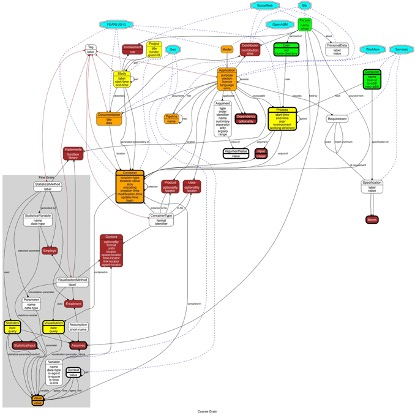
\includegraphics[width=0.48\textwidth]{img/schema.jpeg}
\caption{SSREPI Schema} \label{fig:schema} \end{wrapfigure}

Since the inception of this project, we have subsequently uncovered a similar
project which specifically concentrates on provenance data. This is the FAIR
data pipeline \cite{mitchell2022fair} in which the provenance is automatically
recorded by embedded code in R, C++, Java, Julia and Python.  One of the aims
was not to modify the original code, i.e. the original experiment as unchanged
as possible. That is we wanted to change the framework code rather than the
core code. The core code in the example above being the executable, pre-compiled
in Objective-C \cite{objectivec}. Additionally the support code, i.e. the code
that prepared the data, a Perl \cite{perl563} script and the code that did the
post analysis, a mixture of Perl and R \cite{R422}.  This meant we developed
the database access in Python \cite{python368}, wrote wrapper scripts in Bash
\cite{bash4420}. This differs in approach to [ibid] which is embedded in the
code that constitutes the body of the experiment. Moreover our framework
generalises to more more source metadata (paper, data, other experiments), and
sis written with the requirements of agent-based modelling first and foremost.
That is not to say that we do not have similar ambitions to automatically place
provenance tracing code automatically embedded in experimental model code.

The rest of this paper, we describe the scripting tool we have developed  for
automatically recording metadata, which can be incorporated into the analysis
replication process, and how this  was used to regenerate some of the figures
in \cite{polhill_nonlinearities_2013}. In addition we show a simple tool we have already developed to trace data through the provenance graph, and as usual suggest additional work we would like to pursue and other ideas.


\section{Method}

One of the artefacts of the MIRACLE project \cite{parker2019final} was the
Social Simulation REplication Interface or SSREPI. This is the schema shown in
figure \ref{fig:schema}.  This schema has evolved since it original conception.
The newest version of this document may be found here
\cite{polhill2022miracle}. This is a database schema derived from the Dublin
Core \cite{weibel2000dublin}, the standard XML datatypes \cite{biron2004xml}
and the PROV-O ontologies \cite{missier2013w3c}.  The schema is designed with
agnosticisim towards the underlying database technology and as such has been
implemented both in PostgresSQL \cite{stonebraker1991postgres} and Sqlite3
\cite{sqliteorg2023syntax}.

There are two important dimensions of distinction to this schema. First is
fine- versus coarse- grained metadata. Second is provenance versus workflow.
Coarse-grained metadata describes how particular files come (or came) into
being, or were (or could be) used to bring other files into being. Fine-grained
metadata describes specific values recorded in social simulation outputs. To
make the distinction concrete, suppose a simulation produces a CSV file. The
data within the CSV file are covered by fine-grained metadata, whilst the fact
that the simulation produces the CSV file is coarse-grained. Turning to the
other dimension, provenance metadata describes what actually happens (run W of
simulation X produced output file Y), whilst workflow metadata describes what
could happen (simulation X produces an output file of type Z). The distinctions
are summarised in \ref{fig:finegrain} .

\begin{wrapfigure}{r}{0.5\textwidth}
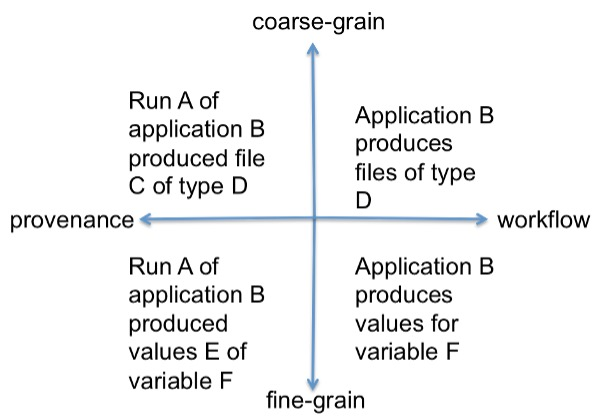
\includegraphics[width=0.5\textwidth]{img/fine-grain-vs-coarse-grain.jpeg}
\caption{Fine grain vs coarse grain provenance} \label{fig:finegrain}
\end{wrapfigure}

Each table in schema shown in fig. \ref{fig:schema} was coded as an object type
in Python. Each table row was represented as an instance of such an object.
This design approach was adopted to enforce a consistent coding methodology
across all tables. 

This then just left the interface between the two scripting languages. The
design decision was taken to do domain specific processing in the Bash
scripting language. This was done for due to the repetitive and time consuming
nature of system testing: amendments in the job control language being easier
to do quickly. This is a decision that may need revisiting. The problem being
that Bash invocations are computationally and time expensive. Complex
processing should be abstracted away from the slower language, in this case job
control language to improve speed and remove what might be regarded as
inappropriate computation for such an environment. Consequently as the system
stands the commands that coordinated between Bash and Python are few and
simple, the harder processing having been pushed down into the job control
level, i.e. in the Bash scripts.

These coordinating commands are:

\begin{itemize} \item {\color{green} \ttvar{create_database.py}} - creates a
        database idempotently.  \item {\color{green} \ttvar{exists.py}} - checks
        if a particular row in a table exists.  \item {\color{green}
            \ttvar{get_value.py}} - gets any specified single value from a
            table given the primary key.  \item {\color{green}
\ttvar{get_values.py}}  - gets one or more rows given the search values. \item {\color{green}\ttvar{next_study.py}} - gets the next available and unique study number. \item
{\color{green} \ttvar{update.py}} - idempotently updates a particular row in a
table.  \end{itemize}

Note the use of idempotent, indicating that multiple operations on
the same entity will leave it unchanged after the initial operation.  For
example multiplying something by 1 is idempotent. This allows for a less
rigorous exception criteria, for instance if a row or entity already exists.
This implies that initialisation must be performed with care, as older data
will not necessarily be destroyed but overwritten with newer values, but
also retaining any values that already exist. Again this design decision was
expedient on rapid development and may need revisiting. However the schema is
and its interaction is quite complex and this would involve critical path
analysis

So each of the Bash commands listed in table \ref{tab:commands} composes over
the above python commands to populate the SSREPI database in a consistent and
logical manner.

For the purposes of this short paper we are concentrating on a demonstration of
recording provenance. Indeed we use the example, mentioned in the introduction
of \cite{polhill2022miracle}, and modified the original Bash \cite{bash4420}
scripts to include the what we denote as \textit{primitives}.  In order to
record provenance we coded the following primitives from the SSREPI interface
definition \cite{polhill2022miracle}. As noted above these are implemented in a
mixture of Python and Bash. 

\tiny \begin{longtable}{|l|p{2cm}|p{7cm}|} \hline Primitive & Type & Purpose \\
    \hline {\color{blue} \ttvar{SSREPI_require\_minimum}} & Metadata & Lower
    bound on software hardware required \\ {\color{blue}
    \ttvar{SSREPI_require\_exact}} & Metadata & Exact bound on software
    hardware required \\ {\color{blue} \ttvar{SSREPI_application}} & Provenance
    \& Metadata & specifies some executable \\ {\color{blue} \ttvar{SSREPI_me}}
    & Provenance \& Metadata & Determines executable being run or returns a
    proper reference to the executable being run. \\ {\color{blue}
    \ttvar{SSREPI_run}} & Provenance \& metadata & Blocking invocation of an
    executable which will allow the specification of all inputs, outputs and
    arguments. Creates run-time provenance information as well \\ {\color{blue}
    \ttvar{SSREPI_batch}} & Provenance \& metadata & Non blocking invocation of
    an executable which will allow the specification of all inputs, outputs and
    arguments. Creates run-time provenance information as well \\ {\color{blue}
    \ttvar{SSREPI_argument}} & Provenance & An argument type to an exectuable
    \\ {\color{blue} \ttvar{SSREPI_output}} & Provenance & An output type from
    an executable \\ {\color{blue} \ttvar{SSREPI_input}} & Provenance & An
    input type for an exectuable \\ {\color{blue}
    \ttvar{SSREPI_hutton\_person}} & Metadata & Uses our institutions databases
    to populate metadata for a given individual \\ {\color{blue}
    \ttvar{SSREPI_person}} & Metdata & Provide metadata for a particular actor
    within this system\\ {\color{blue} \ttvar{SSREPI_project}} & Metadata &
    Specifies a project which contains all studies \\ {\color{blue}
    \ttvar{SSREPI_study}} & Metadata & A set of experiments makes up a single
    study \\ {\color{blue} \ttvar{SSREPI_set}} & Metdata & Sets the default
    licence and other metadata \\ {\color{blue} \ttvar{SSREPI_involvement}} &
    Metadata & Links personnel to a study \\ {\color{blue}
    \ttvar{SSREPI_paper}} & Metadata & A paper associated with this study \\
    {\color{blue} \ttvar{SSREPI_make_tag}} & Metadata & Used for building a
    folksonomy \\ {\color{blue} \ttvar{SSREPI_tag}} & Metadata & Used to tag
    any entity with a folksonomy tag \\ {\color{blue}
    \ttvar{SSREPI_contributor}} & Metadata & A  person with some kind of
    relation to an executable or script. \\

    {\color{blue} \ttvar{SSREPI_statistical_method}} & Metadata & A statistical
    method is an approach to computing some statistics. It may be implemented
    in or as part of an application. A statistical method generates one or more
    statistical variables as its results, and may use the results of another
    statistical method in its computation. For example, computing the standard
    deviation of some data uses the mean of those data. \\ {\color{blue}
    \ttvar{SSREPI_visualisation}} & Metadata & A visualisation is the process
    of creating an image to depict one or more (typically more than one)
    values. The results of a visualisation appear in a container.\\
    {\color{blue} \ttvar{SSREPI_statistics}} & Metadata & Statistics are
    activities that compute  and populate the values of statistical rvariables.
    They operate on raw data that are retrieved from the values using a query.
    To replicate a set of statistics, the query can be rerun, selecting values
    that are pointed to by containers entries \\ {\color{blue}
    \ttvar{SSREPI_visualisation_method}} & Metadata & This describes methods
    for generating visualisations, which then may appear in the content of a
    container produced by a process running an application that implements it.
    \\
    
    {\color{blue} \ttvar{SSREPI_implements}} & Metadata & Links a statistical
    or visualisation method to an application \\ {\color{blue}
    \ttvar{SSREPI_parameter}} & Metadata & A Parameter is the name of a
    parameter taken by a statistical or visualisation method, used to configure
    the way it behaves. \\ {\color{blue} \ttvar{SSREPI_statistical_variable}} &
    Metadata &  A name for (one of) the result(s) of a statistical method. \\
    {\color{blue} \ttvar{SSREPI_visualisation_variable}} & Provenance \&
    Metadata & Declares a named variable of interest \\ {\color{blue}
    \ttvar{SSREPI_variable}} & Metadata & Names a variable of interest \\
    {\color{blue} \ttvar{SSREPI_statistical_variable_value}} & Provenance \&
    Metdata & Sets an actual value for a named statistical variable \\
    {\color{blue} \ttvar{SSREPI_value}} & Provenance & Sets an actual value.
    This can be connected to any metadata value such         \\ {\color{blue}
    \ttvar{SSREPI_content}} & Metadata & Links a kind of output/input/argument
    to a variable  \\ {\color{blue} \ttvar{SSREPI_person_makes_assumption}} &
Metadata & links a person to an assumption \\ \hline \caption{Available Bash
commands for provenance and metadata gathering} \label{tab:commands}
\end{longtable}

\normalsize

Broadly speaking {\color{blue} \ttvar{SSREPI_application}}, {\color{blue}
\ttvar{SSREPI_run}}, {\color{blue} \ttvar{SSREPI_batch}}, {\color{blue}
\ttvar{SSREPI_input}}, {\color{blue} \ttvar{SSREPI_output}} and {\color{blue}
\ttvar{SSREPI_argument}} are responsible for recording coarse grain provenance.
{\color{blue} \ttvar{SSREPI_value}}, {\color{blue}
\ttvar{SSREPI_visualisation_variable_value}}, {\color{blue}
\ttvar{SSREPI_statistical_variable_value}}, {\color{blue} \ttvar{SSREPI_run}}
and {\color{blue} \ttvar{SSREPI_batch}} record fine-grain provenance. The
remaining primitives are largely about recording metadata.

With the tool in the current state this involved laboriously going through the
code and inserting the some of the Bash-based commands, shown in
table \ref{tab:commands}. These commands have a fairly complex parameter set as
it stands, and no way of checking whether the code worked other than running
it, initially on a small subset of the experiment and then scaling up. This was
extremely time-consuming.

Elaboration of all this may be found in the man pages and design documents in
the public repository at \url{https://github.com:/DougSalt/ABM-metadata}.

\begin{figure} \includegraphics[width=\textwidth]{img/workflow.pdf}
\caption{The workflow sub-graph} \label{fig:workflow} \end{figure}

We developed a very basic scheduler for use in an high performance computing
environment, where there are many resources available both on the local
machine. In particular for the situation where they is a single machine that
has a large memory and many cores, the non-blocking version of the  two
execution primitives, specifically {\color{blue} \ttvar{SSREPI_batch}}
implements a kind of a simple scheduler locally using the sub-processing
commands available to Unix-like systems. This was an historical solution to
schedule in an high performance computing environment that existed prior to
clustered computing situations. Clustering is the utilisation of one or more
instances of such powerful computing machinery. Generally schedulers have been
developed for such environments, as such SGE \cite{gentzsch2001sun} and the one
we use as default, Slurm \cite{yoo2003slurm}. Scheduling is now largely handled
outwith the framework, which makes the code less complex.

{\color{blue} \ttvar{SSREPI_run}}, the other executing primitive will block
until the command, code or model is has invoked has completed. This is
necessarily used in single threaded coordination context, such as gathering all
outputs necessary before proceeding to the next stage of processing. For
instance, initial post processing of an all experiments would represent such a
single threaded context.

\section{Results}

The primary result is that the target results and diagrams from the original
paper \cite{polhill2017lessons} were able to be recreated.  As mentioned the
method undertaken in this paper involved inserting the correct Bash-based
commands, listed in table \ref{tab:commands}. These commands have a fairly
complex parameter set as it stands, and no way of checking whether the code
worked other than running it. This led to one of the immediate problems with
this method. The only way to see if the code was working was to run it, a suck
it and see methodology. This was extremely time consuming. We took the obvious
approach and ran small subsets of the ~20,000 runs or so, to see if we could
get the framework to work and then scaled it up to the full run, but invariably
we ran into new problems the more we increased the scale. It therefore took
substantial time to even get this first replication to run. It took several
months of coding effort to get this correct. Generally it would alternate
between parameter errors for the calls in table \ref{tab:commands}, and errors in the scripts making calls to record the provenance data to the database. Each iteration would take weeks to run, before failure as we increased the scale.

After a run had completed successfully the database was run through several
programs to produce the sub-graphs detailed in fig. \ref{fig:schema}. These
programs are capable of producing the following subgraphs:

\begin{itemize} \item \textbf{Analysis} - fine grain provenance pertaining to
            statistical and visualisation outputs.

        \item \textbf{Finegrain} - a provenance diagram down to the level of
        variables.  \item \textbf{Folksonomomy} - a diagram showing annotations
            against the database, produced and categorised at the discretion of
            the user doing the annotation \item \textbf{Project} - management
            metadata. Largest granularity of metadata supported \item
            \textbf{Provenance} - provenance diagram at the level of file and
        parameter \item \textbf{Services} - service provided and requirement
            description \item \textbf{Workflow} - the actual workflow
\end{itemize}

We developed programs that took the relational data in order to produce "dot"
files. Such files that can be processed by Graphviz
\cite{ellson2002graphviz}, and were used to produce the diagrams in figures
\ref{fig:sub-provenance}, \ref{fig:workflow}, \ref{fig:broken-application} and
\ref{fig:high-lit-provenance-trace} .  

To give an idea of the visualisation available we show the workflow graph in
fig. \ref{fig:workflow}. This is a section of the workflow and is relative easy
to follow. The resultant provenance graph is both massive and massively
complex, given there were 20,000 runs (so 20,000 sets of outputs to record), so we only show a \textit{very small} section of the provenance graph in fig.
\ref{fig:sub-provenance}. 

\begin{figure}
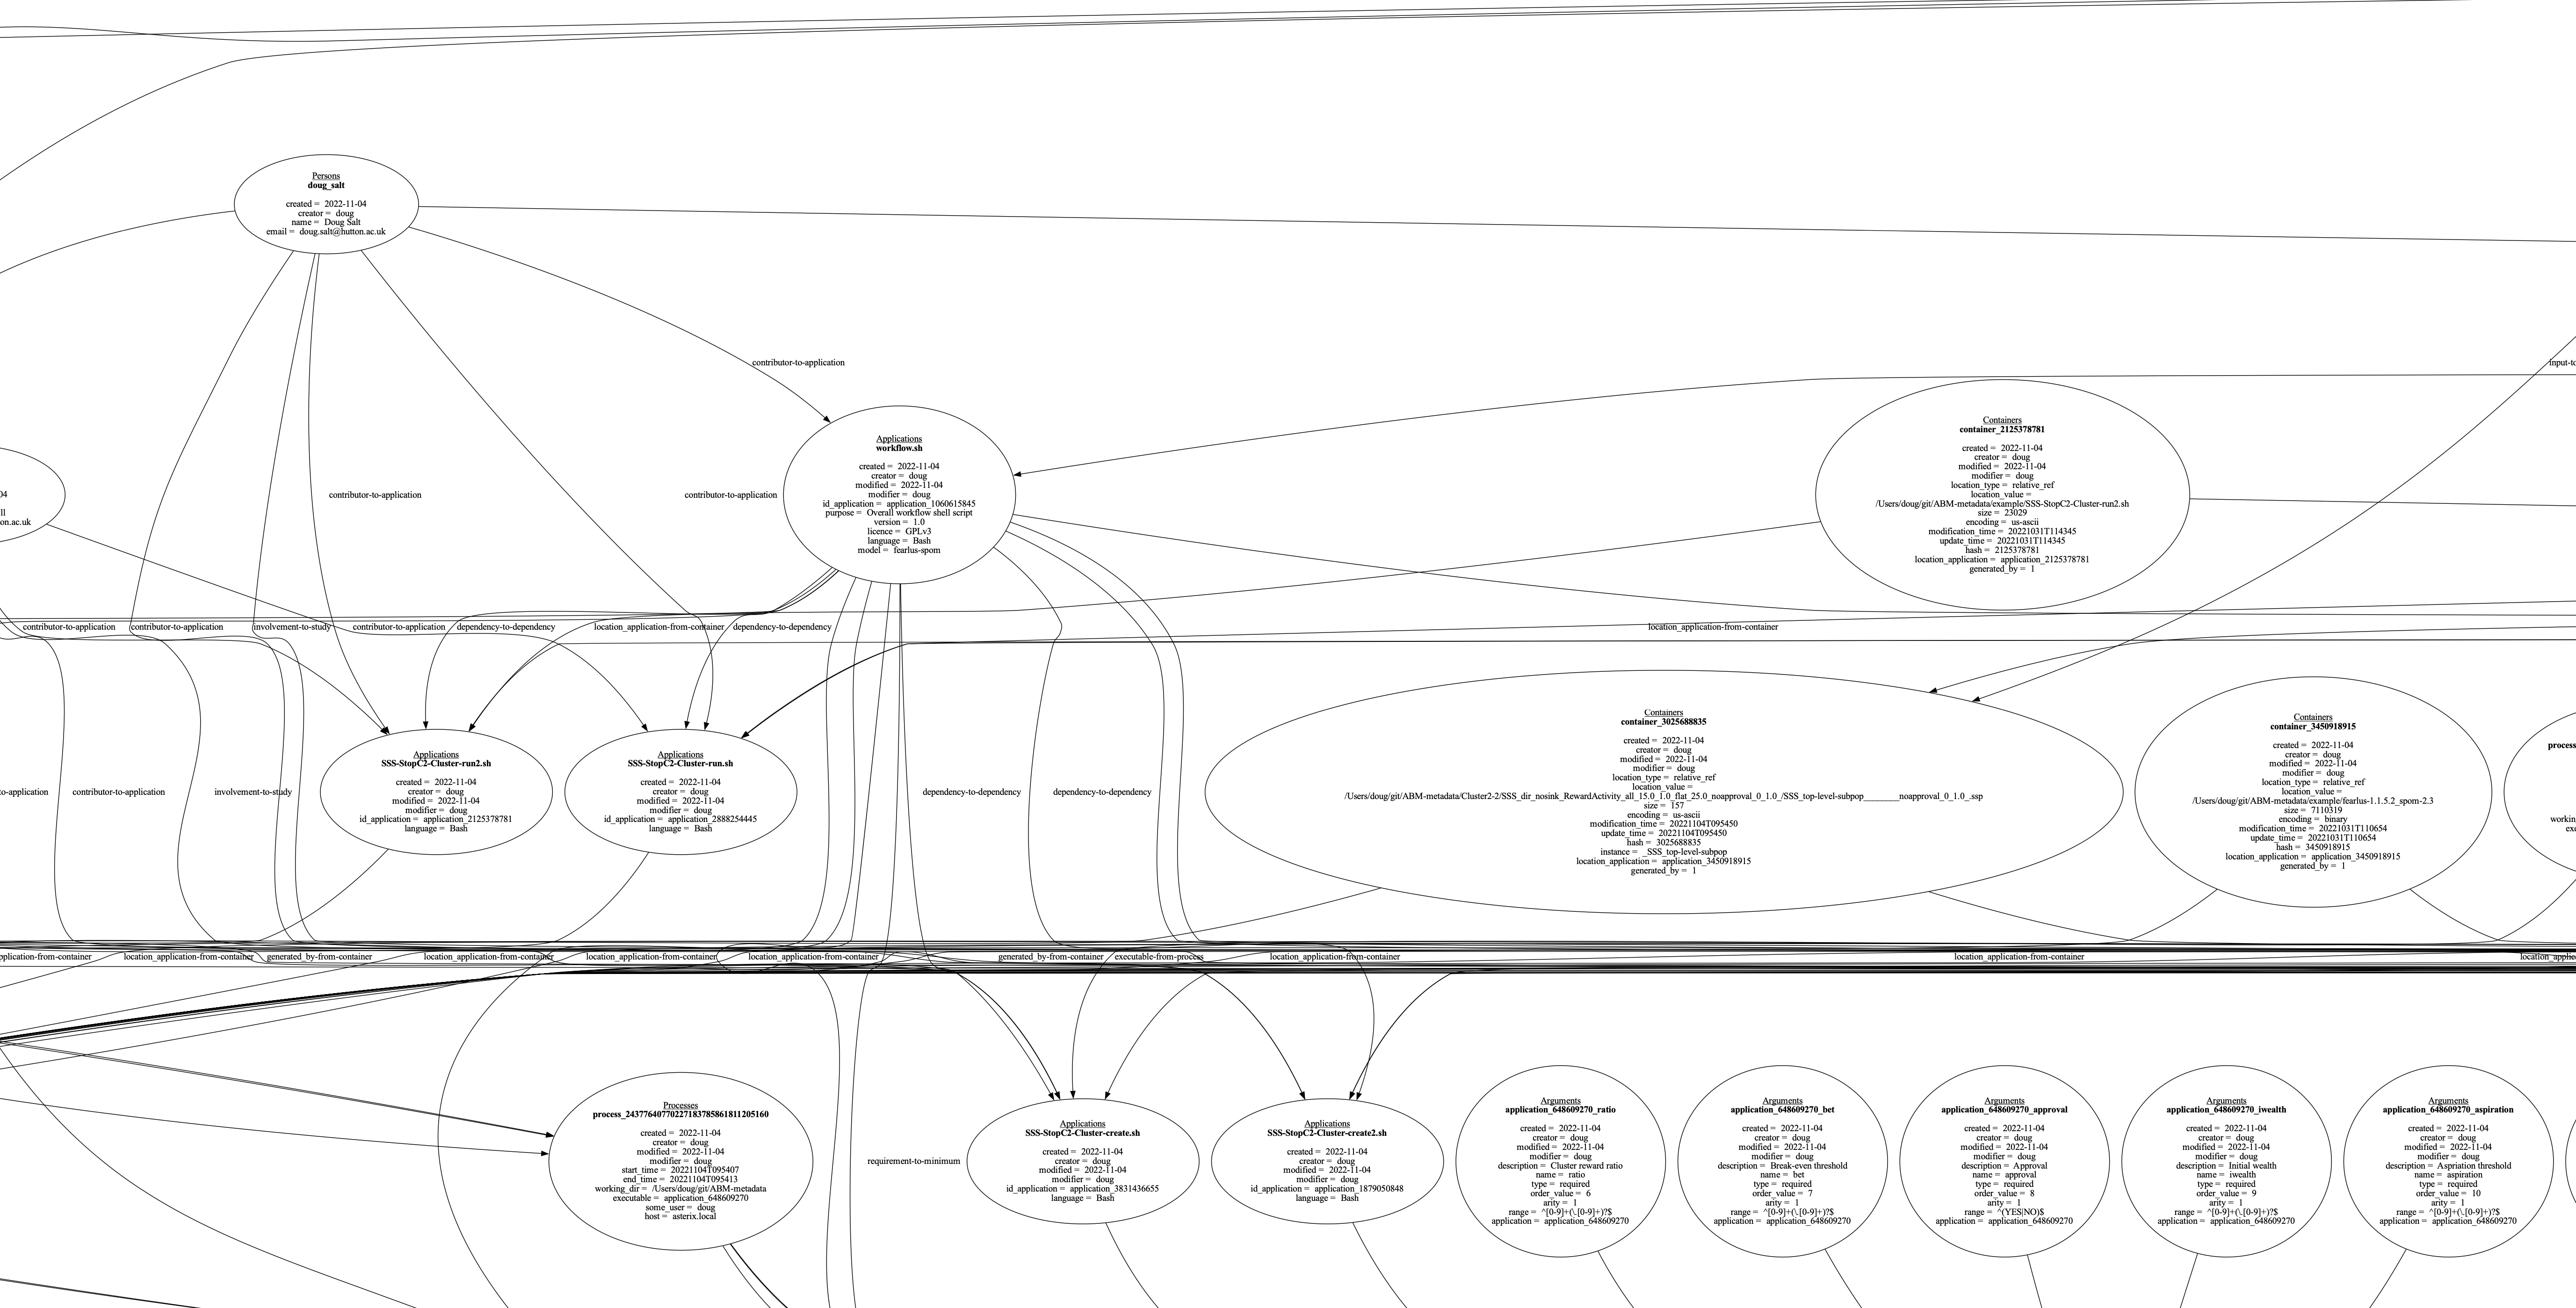
\includegraphics[width=\textwidth]{img/subsection-of-provenance.png}
\caption{A small sub-section of the proevenance graph} \label{fig:sub-provenance}
\end{figure}

So what use is this provenance metadata? Beyond replicability? Say for instance
we have a bad dataset. The challenge is not only how to visualise the
provenance, but to use this data in a useful manner. We propose a simple use
here.  The "dot" language used by Graphviz constitutes a primitive graph
database. Indeed there are programs that can transform "dot" files into
TinkerPop GraphSON format \cite{tinkerpop2015graphson,gv2graphson}. Rather than
using the relational database data we used the resultant dot files listed above
to trace bad entities. \footnote{These are directed graphs (unproven as to
whether they are acyclic - they shouldn't be they are the result of a
relational database which was designed to be and \textit{should} be acyclic).} 

So for an easy to see example we pick the entity {\color{red}\ttvar{Applications.application_3831436655}}, and see how this affects other entities in the graph. This is \ttvar{SSS-StopC2-Cluster-create.pl} and we are using the workflow graph to see what might be affected. And this is shown in \ref{fig:broken-application}. It might be for instance that there is a bug in this program, so we should like to see how the errors might propagate out through the workflow.

\begin{figure} \includegraphics[width=\textwidth]{img/broken-application.pdf}
\caption{The workflow sub-graph} \label{fig:broken-application} \end{figure}

That example was somewhat contrived and simplistic and gives a flavour.
However, what if we wanted to trace a bad data set?  If we ignore for this
original example that the datasets for the above example are generated
automatically by Perl scripts, and we pick one randomly to illustrate how this
approach might work. The dataset in question would be:
{\color{red}\ttvar{Containers.container_42949672955}}, a data file that forms
a input file to just one experiment.  And here we see, again, a \textit{very
small} section of of the provenance graph showing what is affected in red. This
is shown in fig. \ref{fig:high-lit-provenance-trace}

\begin{figure} \includegraphics[width=\textwidth]{img/high-lit-provenance-trace.pdf}
\caption{The workflow sub-graph} \label{fig:high-lit-provenance-trace} \end{figure}

Moreover we can list out the affected entities. In this case, those entities would be:

\tiny

\begin{itemize}
	\item \ttvar{Applications.application_3450918915}
	\item \ttvar{Applications.application_648609270}
	\item \ttvar{Computers.asterix.local}
	\item \ttvar{Containers.container_1814970370}
	\item \ttvar{Containers.container_1982026419}
	\item \ttvar{Containers.container_2050039078}
	\item \ttvar{Containers.container_2056384913}
	\item \ttvar{Containers.container_2060874102}
	\item \ttvar{Containers.container_2387213333}
	\item \ttvar{Containers.container_2486610989}
	\item \ttvar{Containers.container_2582525701}
	\item \ttvar{Containers.container_2759060318}
	\item \ttvar{Containers.container_2865400753}
	\item \ttvar{Containers.container_3025688835}
	\item \ttvar{Containers.container_3307537171}
	\item \ttvar{Containers.container_3470971297}
	\item \ttvar{Containers.container_354343442}
	\item \ttvar{Containers.container_4235735972}
	\item \ttvar{Containers.container_4294967295}
	\item \ttvar{Containers.container_441913555}
	\item \ttvar{Containers.container_505627104}
	\item \ttvar{Containers.container_800277554}
	\item \ttvar{Containers.container_878886043}
	\item \ttvar{Containers.container_900718909}
	\item \ttvar{Persons.doug}
	\item \ttvar{Persons.doug_salt}
	\item \ttvar{Processes.process_23222129888649347509041510897074}
	\item \ttvar{Processes.process_32647549959702293885495865014666}
	\item \ttvar{Specifications.R}
	\item \ttvar{Specifications.bash}
	\item \ttvar{Specifications.cpus}
	\item \ttvar{Specifications.disk_space}
	\item \ttvar{Specifications.memory}
	\item \ttvar{Specifications.os}
	\item \ttvar{Specifications.perl}
	\item \ttvar{Specifications.python}
	\item \ttvar{Studies.1}
	\item \ttvar{Users.doug}
\end{itemize}

\normalsize

\section{Discussion}

What we have learnt from this?  As noted the process of running the experiment
with the new provenance and metadata commands was time-consuming to the point
of almost being unusable. It involved the repeated running of the experiment
with a larger and larger array of inputs until we matched the size of the
original experiment.  This has taken several months of intense work to event get it running. Repeating an experiment in a completely automated fashion turns out to be a really hard task. 

However, we have to emphasise that this was the reproduction of the experiment.
If this framework were available from the start then most of the work would be
done once the experiments had been completed; that is, the work needed to
actually repeat the experiment in a consistent and reliable manner. This is the
key, and it reduces to the same advice that meta-data advocates everywhere
proclaim, which is to incorporate the metadata from the start and not as an
after thought.

Provenance should be a directed acyclic graph. There may well be loops in the
schema as it stands. Given sufficient time we can certainly normalise the
relational database to remove redundancy and the conflict arising from such,
and once this complete,  we can formally prove the schema to be acyclic.  The
authors have done their best to normalise it to uncover such cycles, but have
yet to formally do so. In a schema this complex they may well still exist.
Until the schema is formally analysed, then we can not say with confidence that
the schema is actually consistent, in the sense that any recorded provenance is
not inherently contradictory. Given that such a schema is likely to be
continually revised as the underlying provenance model changes or additional
functionality is required, then it would be advisable to automate such proving
of consistency (assuming correct normalisation).

In addition to reproducing the experiment automatically, there was some scope
in utilising the parallelising infrastructure of the high performance computing
environment.  One of the nice things was that we were able to parallelise part
of the post processing job, and thus speed up the whole experiment as this was
proving to be a bit of a bottleneck. However, careful thought needs to be given
to this. In the case of agent-based modelling such stochasticism in inherent to
the testing methodology, and it would be expected that such changes should have
little impact. For other testing frameworks, particular those that do not rely
on massive replication, then such changes may well have unintended
consequences.  Indeed, those with a sharp eye may have noticed the versions of
Perl, Python and R we use were not around when the original experiments were
run and obviously this has implications. However, the framework does offer the
ability to record and enforce metadata about programming versions.

The underlying database is almost certainly unsuitable. We should probably be
using a graphing language such as Gremlin \cite{rodriguez2015gremlin}. The
advantages of using graphing databases over relational databases is that such
languages are inherently designed to store, traverse and query the graphs that
are the main product of this framework. This makes querying in such languages
trivial and fast. In a relational databases the SQL statement to do this are
cumbersome, awkward and probably error prone given their size. Moreover on huge
datasets they are reportedly slow. Relational databases do have the advantage
of being an extremely mature technology and the availability of utilities that
implies. As mentioned, the advantage of using the relational database is that
structured query language is standard for all such databases, and therefore
queries written for any relational database should be the same. A tool we
already use, Graphviz already does act like a graphing database language to a
certain extent. Indeed we use the Graphviz "dot" files, rather than the
relational schema in our simple tools tools to trace bad data through our
provenance graphs.  However the "dot" language of Graphviz is primarily
purposed as a diagramming language and lacks the sophistication, such as a
built-in query language of say, Gremlin.

For future we work, we should eventually like to take many provenance databases run some machine learning across them to see if there are any commonalities. We hope to uncover similarities in setup, execution and post-processing that could form core, reusable and proven components for primarily agent-based modelling but also for other modelling frameworks.

The plan is to adapt this provenance framework to other model running language
frameworks, in particular R, Python, Julia, Java and thence NetLogo. This would
take the approach of the FAIR data pipeline \cite{mitchell2022fair}, but unlike
the example we have presented here such provenance would be embedded in the
experiments as a matter of course. We were constrained by the nature of the
replication here to use Bash as our means of recording provenance. However this
does show that such a provenance framework may be "retrofitted" to existing
experiments (although possibly at the cost of the programmer's sanity given the
minutiae involved). We have tentative potential adopters using R and Python as their primary modelling language.

% ---- Bibliography ----
%
% BibTeX users should specify bibliography style 'splncs04'.
% References will then be sorted and formatted in the correct style.
%
\bibliographystyle{splncs04}
\bibliography{global.bib}
% \bibliography[keyword={github.com/DougSalt/SSC2023}]{global.bib}
%
\end{document}
